\chapter{Content Mapping}

\label{appendix:content.mapping}

A map based approach inspired by Harry Beck's London Underground tube
map seen in Figure~\ref{figure:beck.1933.map}
(p.~\pageref{figure:beck.1933.map})
will be used for visualizing the navigational relationships between content
items. \citet{walsh07} introduced such visualization methods to the information
architecture field.

\begin{figure}[b]
  \begin{adjustwidth*}{0em}{-\wholemargin}
    \begin{center}
      \label{figure:beck.1933.map}
      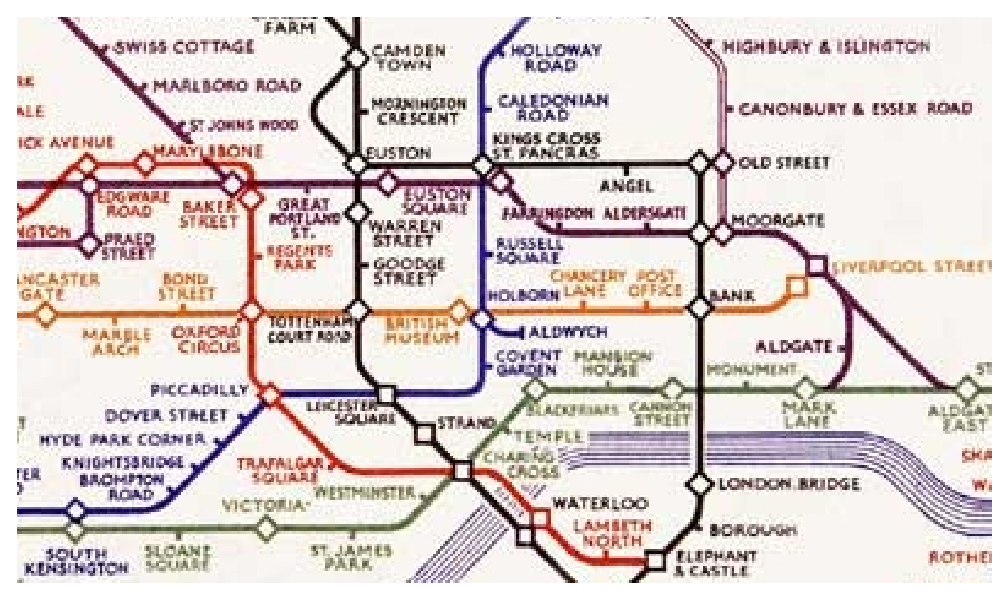
\includegraphics[width=0.9\textwidth]{beck_1933_map}
      \caption[1933 London Underground Tube map]{%
        The present Underground Tube map of London was introduced as early as
        1933 by graphic designer Harry Beck. It's merits are discussed
        with regards to visual design by \citet{hadlaw03} and highlighted as
        a remarkable example of abstraction in relation to computing by
        \citet{kramer07}. Retrieved from the Transport for London web site:
        \url{http://www.tfl.gov.uk/beckmap1.jpg}.}
    \end{center}
  \end{adjustwidth*}
\end{figure}

No maps are available yet since the author don't have access to the required
\emph{Adobe Illustrator} software.
